\documentclass[a4paper, 12pt, final, garamond]{book}
\usepackage{cours-preambule}

\raggedbottom

\makeatletter
\renewcommand{\@chapapp}{Architecture de la mati\`ere -- chapitre}
\makeatother

\begin{document}
\setcounter{chapter}{2}

\chapter{Correction du TD}

\section{Structure cristalline du niobium}
\begin{enumerate}
  \item Un atome sur un des sommets est partagé entre huit mailles et compte
    pour 1/8, l'atome central n'appartient qu'à une seule maille donc
    \[
      \boxed{N = 8\times1/8+1=2}
    \]
  \item La masse d'un atome de niobium est égale à $m_{\ce{Nb}} = M/\Nc_A$,
    masse d'une maille vaut donc $2M/\Nc_A$~; ainsi~:
    \[
      \boxed{\rho = \frac{2M}{\Nc_A a^3} = \SI{8.51e3}{kg.m ^{-3}}}
    \]
  \item La distance entre atomes situés sur deux sommets vaut $a$, celle entre
    atomes situés sur un sommet et au centre de la maille vaut $a \sqrt{3}/2 <
    a$~: le contact a donc lieu \textbf{le long de la grande diagonale} du cube.
    Ainsi, en comptant successivement les atomes,
    \[
      a \sqrt{3} = r+2r+r
      \qqdonc
      \boxed{r = a \frac{\sqrt{3}}{4} = \SI{143}{pm}}
    \]
  \item La compacité est la proportion du volume de la maille réellement occupé
    par la matière. Pour la structure CC,
    \[
      C = \frac{2\times \frac{4}{3}\pi r^3}{a^3} = \frac{8\pi}{3}\times \left(
      \frac{\sqrt{3}}{4} \right)^{3}
      \qqdonc
      \boxed{C = \frac{\pi \sqrt{3}}{8} = \num{0.68}}
    \]
\end{enumerate}

\section{Galène}
\noindent
\begin{minipage}[t]{.6\linewidth}
  \begin{enumerate}
    \item Voir figure.
    \item En raisonnant sur un cation, par exemple au centre du cube, ses PPV sont
      sur les faces du cube (et forment l'octaèdre), distants de $a/2$~: les
      cations ont une coordinence de 6. \smallbreak
      En raisonnant sur un anion, par exemple au centre de la face avant, ses PPV
      sont les cations aux centres des arêtes (donc 4) \textbf{plus} les cations
      au centre des 2 mailles auquel cet anion appartient. Ainsi, les anions ont
      également une coordinence de 6.
  \end{enumerate}
\end{minipage}
\hfill
\begin{minipage}[t]{.3\linewidth}
  ~
  \begin{center}
      \vspace*{-10pt}
      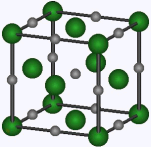
\includegraphics[scale=1]{galene}
      \captionof{figure}{Maille élémentaire de la galène. Les anions sont en vert,
      les cations en gris.}
      \label{fig:gal}
  \end{center}
  
\end{minipage}
\begin{enumerate}[resume]
  \item La population d'une maille CFC est de $8\times1/8+6\times1/2=4$, donc on
    a 4 anions \ce{S^{2+}} en propre. On a également 4 sites O en propre
    $(1+12\times1/4)$, donc 4 cations \ce{Pb^{2+}}. Ainsi, la masse volumique
    vaut
    \[
      \rho = \frac{4M_{\ce{Pb}} + 4M_{\ce{S}}}{\Nc_A a^3}
      \qqdonc
      \boxed{a = \left( \frac{4(M_{\ce{Pb}} + M_{\ce{S}})}{\Nc_A\rho}
      \right)^{1/3} = \SI{596}{pm}}
    \]
\end{enumerate}

\section{Trioxyde de tungstène}
\begin{enumerate}
  \item Voir figure. On a $8\times1/8 = 1$ cation \ce{W^{+6}}, et $12\times1/4 =
    3$ anions \ce{O^{2+}}, d'où la stœchiométrie.
    \begin{figure}[h]
      \centering
      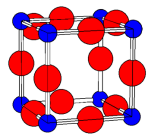
\includegraphics[scale=1]{tungstene}
      \caption{Maille élémentaire du trioxyde de tungstène. Les anions sont en
      rouge, les cations en bleu.}
      \label{fig:tung}
    \end{figure}
  \item Contact anion-cation sur une arête, soit $a = r_{\ce{W}} + 2r_{\ce{O}} =
    \SI{338}{pm}$. D'où la compacité,
    \[
      \boxed{
        \frac{
          \frac{4}{3}\pi r_{\ce{W}}^{3} + 3\times \frac{4}{3}\pi
            r_{\ce{O}}^{3}}{
          (2r_{\ce{W}} + 2r_{\ce{O}})^{3}
        }
        = \num{0.51}
      }
    \]
  \item Les anions \ce{O^{2-}} ont un rayon ionique supérieur aux cations
    \ce{W^{6+}}~: ce sont eux qui contraignent l'habitabilité. Pour loger un
    hétéroélement au centre d'une face, il faut que son rayon $r$ soit tel que
    \[
      2r_{\ce{O}} + 2r \leq a
      \qqsoit
      \boxed{r \leq \frac{a}{2} - r_{\ce{O}} = \SI{62}{pm}}
    \]
    Pour loger un hétéroélement au centre du cube, la contrainte est imposée par
    les anions au centre de deux arêtes opposées le long de la diagonale
    du cube (dans le plan à $z = a/2$). Ainsi,
    \[
      2r_{\ce{O}} + 2r \leq a \sqrt{2}
      \qqsoit
      \boxed{r \leq \frac{a \sqrt{2}}{2} - r_{\ce{O}} = \SI{142}{pm}}
    \]
  \item \ce{H+} pourrait s'insérer dans les deux types de sites, mais les autres
    cations alcalins ne peuvent s'insérer \textbf{qu'au centre du cube}.
\end{enumerate}

\section{Alliages du cuivre}
\begin{enumerate}
  \item Voir cours~: $N = 8\times1/8 + 6\times1/2 = 4$. Dans une maille CFC, il
    y a contact le long de la diagonale d'une face~; ainsi,
    \[
      a \sqrt{2} = 4r_{\ce{Cu}}
      \qqdonc
      \boxed{a = \frac{4r_{\ce{Cu}}}{\sqrt{2}} = \SI{361}{pm}}
    \]
  % TODO: schéma exercice
  \item 
    \begin{enumerate}
      \item Schéma à faire. La maille compte $8\times1/8 = 1$ atome d'argent, et
        $6\times1/2 = 3$ atomes de cuivre~; l'alliage est donc \fbox{\ce{Cu_3Ag}}.
      \item Contact entre atomes le long de la diagonale d'une face, donc
        \[
          a' \sqrt{2} = 2r_{\ce{Cu}} + 2r_{\ce{Ag}}
          \qqdonc
          \boxed{a' = \SI{385}{pm} > a}
        \]
        ce qui est logique puisque le rayon métallique de l'argent est supérieur
        à celui du cuivre. La masse volumique vaut
        \[
          \boxed{\rho' = \frac{3M_{\ce{Cu}} + M_{\ce{Ag}}}{\Nc_A a'^{3}} =
          \SI{8.71e3}{kg.m^{-3}}}
        \]
    \end{enumerate}
  \item 
    \begin{enumerate}
      \item Voir figure. On compte $8\times1/8 = 1$ atome de cuivre par maille,
        et 1 atome de zinc, d'où \fbox{\ce{CuZn}}.
        \begin{figure}[h]
          \centering
          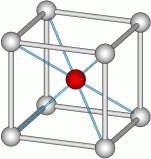
\includegraphics[scale=1]{laiton}
          \caption{Maille élémentaire du laiton. Le cuivre est en gris, l'atome
          de zinc en rouge.}
          \label{fig:laiton}
        \end{figure}
      \item Contact le long de la grande diagonale~:
        \[
          a'' \sqrt{3} = 2r_{\ce{Cu}} + 2r_{\ce{Zn}}
          \qqdonc
          \boxed{a'' = \SI{303}{pm}}
        \]
        et la masse volumique vaut
        \[
          \boxed{\rho'' = \frac{M_{\ce{Cu}} + M_{\ce{Zn}}}{\Nc_Aa''^{3}} = \SI{7.71e3}{kg.m ^{-3}}}
        \]
    \end{enumerate}
  \item On constate à partir des résultats précédents que les mailles sont
    déformées dans les alliages. Ceci a un effet sur la facilité de
    déplacement des électrons de conduction au sein du cristal, et donc sur ses
    propriétés de conduction électrique macroscopique. La présence
    d'hétéroélements rend plus difficile le glissement des plans de cations les
    uns sur les autres dans le matériau, ce qui explique la modification des
    propriétés mécaniques.
    
\end{enumerate}

\section{Structure d'un alliage du titane}
\begin{enumerate}
  \item Voir figure.
    \begin{figure}[h]
      \centering
      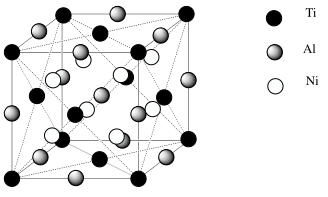
\includegraphics[scale=.8]{titane_alliage}
      \caption{Maille élémentaire de l'alliage. Les couleurs sont indiquées dans
      la légende.}
      \label{fig:titall}
    \end{figure}
  \item Dans une structure CFC, il y a autant de sites O que d'atomes par
    maille, et deux fois plus de sites T que d'atomes par maille. Ainsi, la
    formule de l'alliage est~:
    \[
      \boxed{\ce{AlNi_2Ti}}
    \]
  \item L'arête est de longueur $a = \SI{589}{pm}$. On trouve les sites O au
    milieu de l'arête. La condition de tangence s'écrit donc~:
    \[
      a = 2 (r_{\ce{Ti}} + r_{\mathrm{O}})
      \qqdonc
      \boxed{r_{\mathrm{O}} = \frac{a}{2} - r_{\ce{Ti}} = \SI{147.5}{pm}}
    \]
    ce qui est effectivement suffisant pour l'aluminium. Le site T est sur la
    grande diagonale des petits cubes d'arête $a/2$, d'où
    \[
      a \frac{\sqrt{3}}{2} = r_{\ce{Ti}} + 2r_{\mathrm{T}} + r_{\ce{Al}}
      \qqdonc
      \boxed{r_{\mathrm{T}} = \frac{1}{2} \left( a \frac{\sqrt{3}}{2} -
      r_{\ce{Ti}} - r_{\ce{Al}} \right) = \SI{110}{pm}}
    \]
    ce qui est un peu faible pour l'atome de nickel.
  \item $C$ est le rapport volume occupé/volume de la maille~:
    \[
      C = \frac{4\times \frac{4}{3}\pi r_{\ce{Ti}}^{3} + 4\times \frac{4}{3}\pi
      r_{\ce{Al}}^{3} + 8\times \frac{4}{3}\pi r_{\ce{Ni}}^{3}}{a^3}
      = \frac{16\pi}{3a^3} \left( r_{\ce{Ti}}^{3} + r_{\ce{Al}}^{3} +
      r_{\ce{Ni}}^{3} \right) = \num{0.813}
    \]
    et pour la masse volumique~:
    \[
      \rho = \frac{4 (M_{\ce{Ti}} + M_{\ce{Al}} + 2M_{\ce{Ni}})}{\Nc_Aa^3}
           = \SI{6250}{kg.m ^{-3}}
    \]
  \item L'alliage est utilisé car notablement moins dens, donc la masse des
    appareils s'en trouve réduite.
\end{enumerate}

\section{Carboglace}
\begin{enumerate}
  \item Le dioxyde de carbone a une géométrie \textbf{linéaire}.
  \item 
    \begin{enumerate}
      \item La maille est ci-après. On a $8\times1/8+6\times1/2 = 4$ molécules
        de \ce{CO2} par maille.
        \begin{figure}[h]
          \centering
          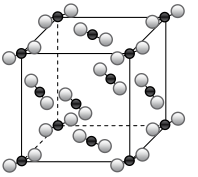
\includegraphics[scale=.8]{carboglace}
          \caption{Maille élémentaire de carboglace. Le carbone est en noir,
          l'oxygène en gris.}
          \label{fig:cbgl}
        \end{figure}
      \item Selon la diagonale d'une face, $2d = a \sqrt{2} \Ra \fbox{d =
        \SI{395}{pm}}$. Cette distance est la somme d'une longueur de liaison
        covalente \ce{C=O} (\SI{120}{pm}) et d'une distance entre \ce{O} d'une
        molécule et \ce{C} d'une molécule voisine~: celle-ci vaut donc
        \SI{275}{pm}, soit nettement plus que la longueur d'une liaison
        covalente. En effet, la cohésion entre molécules de \ce{CO2} est assurée
        par des forces de Van der Waals, d'énergie plus faible qu'une liaison
        covalent.
    \end{enumerate}
  \item La compacité est le rapport du volume occupé sur le volume de la maille.
    Ainsi, avec $N_{\ce{O}} = 8$ et $N_{\ce{C}} = 4$, on a
    \[
      C = \frac{N_{\ce{C}}\times \frac{4}{3}\pi r_{\ce{C}}^{3} +
      N_{\ce{O}}\times \frac{4}{3}\pi r_{\ce{O}}^{3} }{a^3} = \num{0.12}
    \]
  \item La masse volumique est
    \[
      \rho = \frac{N_{\ce{C}}M_{\ce{C}} + N_{\ce{O}}M_{\ce{O}}}{\Nc_A a^3}
      = \SI{1.68e3}{kg.m ^{-3}}
    \]
    La densité, rapport de la masse volumique de la carboglace sur la masse
    volumique de l'eau, est donc \fbox{$d = \num{1.68}$}.
\end{enumerate}

\end{document}
